\documentclass{article}
\usepackage[utf8]{inputenc}
\usepackage{natbib}
\usepackage[T1]{fontenc}
\usepackage[francais]{babel}
\usepackage{chemist}
\usepackage{array}
\usepackage[version=3]{mhchem}
\usepackage{amsmath}
\usepackage[squaren,Gray]{SIunits}
\usepackage{numprint}
\usepackage{amsfonts}
\usepackage{amssymb}
\usepackage{graphicx}
\usepackage{mathtools}
\usepackage{fullpage}
\usepackage{mhchem}
\usepackage{listings}
\usepackage{hyperref}
\usepackage{mathenv} %%%%%%%%%%% do not forget to add to head.tex
\usepackage{empheq} %%%%%%%%%%%% same
\author{Groupe 1246 }


\begin{document}
\title{Rapport de la tâche 7: Yara-Tertre}
\maketitle
\newpage
\section*{L'entreprise Yara}
L'entreprise Yara est une société chimique multinationale, dont le siège social est basé en Norvège. C'est une des entreprises phare dans la production d'engrais azotés sous forme cristalline. Elle est aussi importante dans le domaine de la production d'ammoniac.
\section*{Le site de Tertre}
On peut se demander pourquoi l'entreprise Yara a choisi Tertre comme lieu d'implentation pour son site de production d'ammoniac. Cela est en fait dû à l'emplacement stratégique: l'unité est placée à un croisement de voies marchandes de gaz naturel. En effet, les procédés ayant une consommation moyenne de $\unit{12 \cdot 10^5}{\meter^3\per jour}$ de gaz naturel (la consommation annuelle du centre de Tertre représente $\approx 2\%$ de la consommation annuelle belge de gaz naturel), un bon moyen d'apport en gaz naturel n'est pas négligeable. Les principaux pays d'importation sont la Russie et la Norvège. La production d'ammoniac n'est pas le domaine principal d'activité sur le site de Terte, mais est en fait une partie d'une chaine de production d'engrais sous forme de granulés. À titre d'information, le site produit environ $\unit{10^6}{\tonne\per an}$ d'engrais. Cela correspond à une production moyenne journalière de $NH_3$de $\unit{1100}{\tonne\per jours}$. Les batîments étant vétustes, cette quantité de production est limitée comparée à celle d'une unité de production de dernière génération qui peut atteindre $\unit{3000-3500}{\tonne\per jours}$. 
\subsection*{Flowsheet simplifié des procédés}
\begin{center}
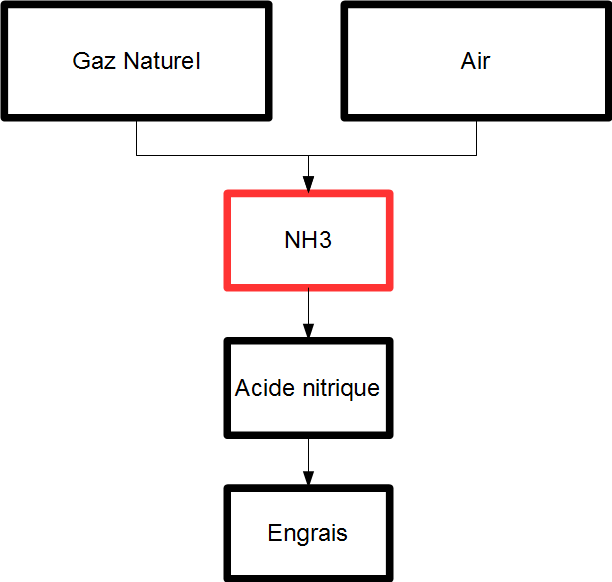
\includegraphics[scale=0.6]{FlYara.png}
\end{center}

\newpage
\section*{Stockage de l'ammoniac}
\subsection*{Engrais}
Les différents engrais sont stockés sous formes de granulés solides, eux-mêmes stockés sous formes de grands sacs appelés "big-bags" (\unit{600}{\kilogram}). A titre d'information, lors des journées de grande production, 250 camions sortent de l'usine remplis de big-bags. 
\subsection*{Ammoniac}
Tout d'abord voici quelques propriétés intéressantes concernant l'ammoniac:

\begin{itemize}
\item{$T_{critique} = \unit{132.4}{\celsius}$}

\item{Point d'ébullition = $\unit{-33.43}{\celsius}$}

\item{Point de fusion = $\unit{-77.76}{\celsius}$}
\end{itemize}

Deux procédés sont utilisés dans le stockage de l'ammoniac: la cryogénisation et la pressurisation. Dans le premier, l'ammoniac produit est refroidit en dessous de $\unit{-33.43}{\celsius}$ pour être obtenu sous forme liquide. Dans le second, l'ammoniac est pressurisé jusque à une pression de $\unit{10-15}{bars}$, à une température de $\unit{20}{\celsius}$. A Tertre, c'est principalement le type de stockage par cryogénisation qui est utilisé. L'ammoniac sous forme aqueuse obtenu est ensuite stocké dans des réservoirs appelés "tanks" ayant une capacité de \unit{15000}{\tonne}. De plus, la forme de ces "tanks" est sphérique lorsque le type de stockage utilisé est celui par pressurisation.


\section*{Rendement et utilisation de catalyseurs}
Le rendement moyen de l'unité de production d'ammoniac est de $\approx 15-16\%$ en fin de chaîne. L'utilisation de catalyseurs est d'une importance capitale. En effet, celle-ci va considérablement faciliter l'obtention d'un milieu réactionnel propice:

\begin{figure} [h]
\begin{center}
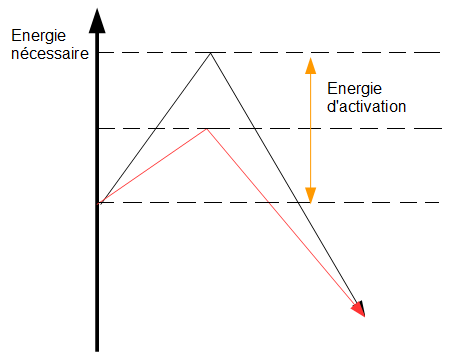
\includegraphics[scale=0.5]{schrend}]
\end{center}
\end{figure}

On remarque que la courbe rouge (celle de l'énergie nécessaire à la réaction avec la présence d'un catalyseur) est nettement inférieure à la noire. L'utilisation d'un catalyseur permet donc de diminuer l'énergie d'activation de la réaction, avec l'avantage de ne pas modifier cette dernière. A titre d'exemple, pour réaliser la réaction de synthèse de l'ammoniac sans catalyseurs afin d'atteindre de mêmes proportions de production que celles de l'unité de production de Tertre, il faudrait que le milieu réactionnel soit porté à une température de $\unit{1000}{\celsius}$ à une pression de $\unit{2000}{bars}$. Malgré tout, le rendement atteint à Tertre ne le serait pas dans de telles conditions.

\subsubsection*{Energie d'activation}
L'énergie d'activation est l'énergie nécessaire pour qu'une réaction chimique puisse s'établir. Une expression de celle-ci peut être établie en partant de la loi d'Arrhenius:

$$k=A\cdot e^{\dfrac{-E_a}{RT}}$$

avec $A$ le coefficient pré-exponentiel, $R$ la constante des gaz parfaits, $T$ la température en Kelvin, $E_a$ l'énergie d'activation et $k$ la constante de vitesse.
On obtient, lorsqu'on travail avec deux températures, grâce un artifice de calculs:

$$\ln(k) = \ln(A) - \dfrac{E_a}{RT}   \Rightarrow   \ln(k_2) - \ln(k_1) = \left( ln(A) - \dfrac{E_a}{RT_2} \right) - \left( \ln(A) - \dfrac{E_a}{RT_1} \right)$$

et au final:

$$E_a = \dfrac{\left( \ln \left( \dfrac{k_2}{k_1}\right) \right) \cdot R}{\dfrac{1}{T_1} - \dfrac{1}{T_2}}$$

\subsection*{Explication simplifiée du fonctionnement d'un catalyseur}
Il nous a été expliqué que les catalyseurs pouvaient être représentés comme des matériaux porreux dont les cavités étaient des endroits réactionnels propices à la réaction:

\begin{figure} [h]
\begin{center}
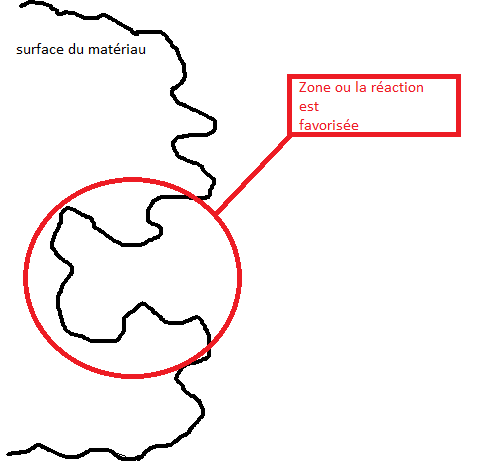
\includegraphics[scale=0.5]{cata}]
\end{center}
\end{figure}

Les catalyseurs utilisés à Tertre sont formés en général à base de nickel et d'arsenic et ont une durée de vie qui est estimée à 12 ans.

\section*{Problèmes et dangers potentiels}
Le centre de production d'ammoniac comporte de multiples dangers potentiels qui doivent être gérés. 

\subsection*{Exothermie des réactions}
Une des difficultées majeures à gérer est l'exothermie de certaines réactions. Par exemple, dans ce cas-ci, celle du réacteur primaire. Au centre de production de Tertre, cette réaction se produit aux alentours de $\unit{1000}{\celsius}$. Il a fallu développer des alliages spécifiques afin d'assurer la résistance des différentes installations. Un autre avantage des alliages est le fait que ceux-ci résistent mieux à la corrosion hydrogénique qui pourrait apparaitre dans certaines conditions, dont la réaction est la suivante:

\ce{{Fe_{3}C}_{(s)}+2H_{2(g)} \Rightarrow CH_{4(g)} + 3Fe_{(aq)}}

\subsection*{Arrêt de production et manque de certains composants}
Un problème apparait dans la phase d'arrêt de production: le manque de vapeur sur les catalyseurs. Ceux-ci, quand il ne sont plus en présence de vapeur, vont réagir et une couche de carbone va se former à leur surface. Le matériau devient une sorte de charbon. Le problème est le suivant: en se transformant, ils deviennent une sorte de bouchon dans les tuyaux. La chaîne est alors complétement arrêtée afin d'éviter tout autre problème qui pourrait surgir suite à l'apparition de ces bouchons. La seule façon de pouvoir relancer la mécanique est de remplacer les tuyaux défectueux. Le problème est que ceux-ci doivent-être commandés longtemps à l'avance et coûtent cher à l'unité.

\subsection*{Impact environnemental}
L'impact environnemental du procédé est l'une des préocupations principales de la société Yara. La production d'ammoniac génère une quantité non négligeable de polluants tels que du \ce{CO_2}, de l'arsenic, du nickel, des oxydes d'azote mais aussi de l'huile provenant des fuites des machines tournantes. Contrairement à ce que l'on pourrait penser, ce sont les oxydes d'azote
qui polluent le plus, ils sont proportionellement plus néfastes pour la couche d'ozone que le \ce{CO_2}, c'est pourquoi Yara est particulièrement attentif au rejet de ce composé. Une production journalière de $\unit{1100}{\tonne}$ de \ce{NH_3} génère pas loin de $\unit {1000}{\tonne}$ de \ce{CO_2} dont $50 \%$ sera revendu à des sociétés tel que ABinbev ou Coca-Cola pour gazéifier leur boissons. Il est évident que le sol du site sera également contaminé par d'éventuelles fuites d'huile ou des produits de nature quelconque, et que cela necessitera donc une dépollution du site à la fin de l'activité industrielle sur celui-ci. L'utilisation des catalyseurs notamment à base d'arsenic ou de nickel nécessite également un traimtement bien particulier afin de préserver l'environnement. Il est évident que cette liste de polluants est non exhaustive dans le cadre d'une installation industrielle de la taille de celle de Yara à Tertre mais par le biais de ces quelques exemples ci-dessus nous pouvons nous rendre comptre de l'impact d'un tel procédé sur l'environnement et de ce que cela implique au niveau du traitement des déchets.

\end{document}
